\documentclass[a4paper, 12pt]{article}
\usepackage{amsmath}
\usepackage{amsthm}
\usepackage{amssymb}
\usepackage{longtable}
\usepackage{pdflscape}
\usepackage{algorithm}
\usepackage{graphicx}
\usepackage{float}
\usepackage[noend]{algpseudocode}
\usepackage{url}
\usepackage{tikz}
\usetikzlibrary{arrows}
\usepackage{float}

\newlength\tindent
\setlength{\tindent}{\parindent}
\setlength{\parindent}{0pt}
\renewcommand{\indent}{\hspace*{\tindent}}

\newtheorem{thm}{Theorem}
\newtheorem{cor}{Corollary}[thm]
\newtheorem{lemma}{Lemma}[thm]

\title{NWEN 303 Project 1}
\author{Daniel Braithwaite}

\begin{document}
	\pagenumbering{gobble}
	\maketitle
	\newpage
  	\pagenumbering{arabic}
  	
	\section{Design Of Program}
		\subsection{Purpous Of Classes}
			\begin{enumerate}
				\item \textbf{Maze:} The maze class encapsulates our representation of the maze. It handles getting the neighbors of a cell and provides static methods for filtering the neighbors based on markings they may or may not have.
				
				\item \textbf{MazeCell:} Encapsulates a cell in the maze, position and type. Stores the search party's currency at that cell. Holds all the markings given to that cell.
				
				\item \textbf{SearchParty:} Extends the thread class, the run method handles moving the search party through the maze and spitting the party up if necessary.

				
				\item \textbf{RetraceParty:} Only used the first time a search party finds the finish. Simply retraces steps to find the start marking each cell as gold as it goes. Once it reaches the start it creates a new search party sending the person back to the finish.
				
			\end{enumerate}
			
		\subsection{Creation Of Processes}
			New processes are created when a search party arrives at a junction where there are multiple unexplored options. This works by dividing the number of people between all the possible choices, and starting a new search party (process) to explore this path. If the original party doesn't have enough people to cover all the paths then it will split up over as many as it can.\\
			
			When a search party finds the exit, if it was the first then a single person (new process) traces the path back to the start, Once the path has been retraced then the person creates a new search party to get back to the finish.
		
		\subsection{Description of Joining Processes}
			Each maze cell keeps track of which search party's (processes) are currently in it. Before a search party makes a decision about what to do next it will check whether another search party has attempted to join with it. Setting up a join is not an atomic operation so we use locks to ensure that if one search party is preparing to join with another, no other process is allowed to access the list of processes in the maze cell. This also means that the process being joined with cant check to see if a join has been requested until the request has been finished.\\
			
			If a join is successful then the process which received the request updates the number of people in the other process, signals the other process (saying the join is complete) and finally terminates.\\
			
			We now arrive at a problem, what happens if a process makes a decision about what to do but then before it can remove its self from the maze cell another process attempts a join. It doesn't make sense for this join to be successful because then we would have to go back and reverse the operations we just performed. So before a process removes its self from a cell it needs to check if a join was attempted, if there was it needs to signal that process so we don't end up with processes waiting for ever and never reaching the finish.
			
		\subsection{Shared Data}
			The maze and maze cells are the shared pieces of data in this program. And the only time this sharing becomes an issue is when we are accessing the markings of a maze cell, when a search party reaches the finish and we are recording that people have reached the end and when we are joining two search party's. Currently all methods modifying the markings of a maze cell is synchronized, and any process which is updating the number of finished people must acquire a lock first. Now we examine the race conditions caused by removing the locks to see if it is possible to remove them.
			
			\subsubsection{Maze Cell Markings}
  				The only time this race condition could potentially be an issue is at junctions, and if two search party's arrive at a junction at the same time then one attempts to join the other, forcing that process to wait until its signaled. It will only be signaled after the other process has finished modifying the junction or after a join has occurred. In ether case we only have one process modifying the maze cell at a time.
  	
			\subsubsection{Finishing Search Party's}
				If we don't put a lock then we could have a situation where two processes reach the finish at the same time, when they both ask if they are the first the answer is yes, then they both send someone to retrace the path taken through the maze. This doesn't matter as both will take the same path adding the same marking to each cell. However there is a more sinister read-modify-write race condition where if two process update the number finished at the same then only one update might get recorded. So we cant remove the use of locks here.

			
			\subsubsection{Joining Search Party's}
				Here we must use locks, as they stop will block other processes from making a decision while they are being joined with.
				
		
  	
	\section{guaranteeing Solution}
		\subsection{Path To Goal}
			The solution outlined above doesn't guarantee that a solution will always be found. When there is a small number of people and there isn't always enough to split up to explore every avenue at once there is the possibility that all the people get stuck in a loop and thus cant find the exit. We would like to use something simple like the left (or right) hand wall follow but we cant because the map can contain cycles. So to solve this issue whenever we arrive at a junction and the search party only contains 1 person then we choose the direction at random. If we can assume a uniform distribution of random numbers then eventually we are guaranteed to explore every path and find the solution.	
			
		\subsection{All Find Finish}
			It is possible for a process to get stuck in a dead end depending on the order of execution of processes. If a process splits up to explore two avenues (both dead ends), before one gets execution time the other thread comes along and marks everything around it as being a dead end then when it finally gets execution time it is stuck. To solve this issue we store the arrival direction not only at junctions but at every cell, this way if a process gets to a state where it only has dead neighbors we can re trace our steps to arrive at that cell until we reach a place with at least one neighbor that isn't dead.
		
  	
  	\section{Base Solution}
		To see how this solution performs we run it with a total number of people ranging from 1 to 20. For each number of people we average our data point over 50 iterations.
		
		\begin{figure}[H]
			\centering
			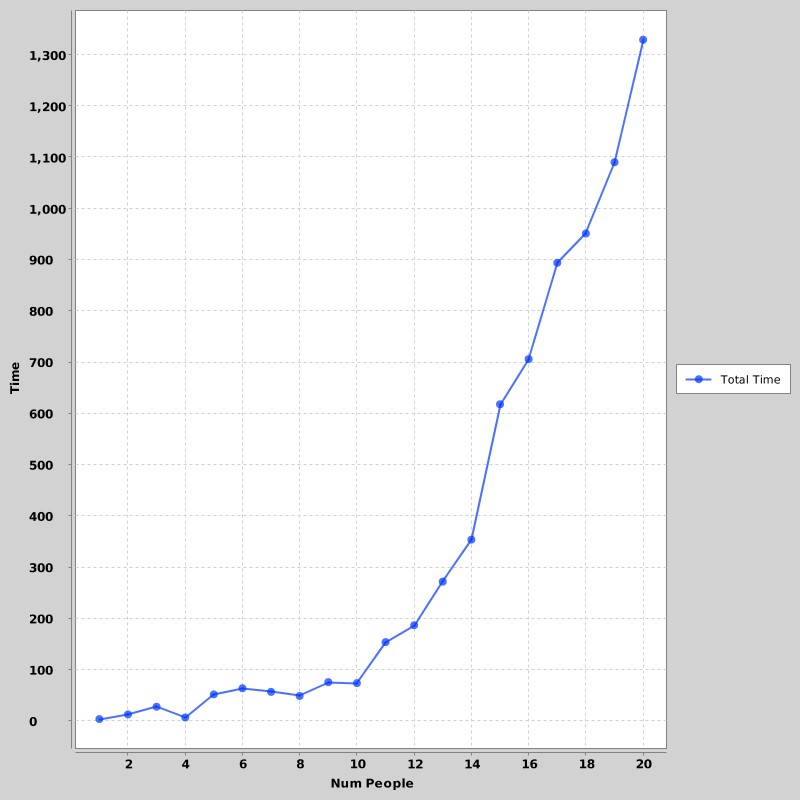
\includegraphics[scale=0.4]{numpeople-vs-time(base-solution)}
			\caption{number of people vs time taken to solve maze for the base solution}
		\end{figure}
		
		The graph has a clear trend, the time taken to solve the maze greatly increases as the number of people increases
  	

	\section{Solution Modifications}
		\subsection{Split For Unvisited}
			Currently when ever a search party arrives at a junction we split the party over each of the non dead neighbors. Instead of doing this we only split up the party at a junction if there are multiple unvisited party's. This reduces the number search party's (processes), and thus the number of search party's we have to wait for when a solution has been found is smaller. We decide which path to take by making a random decision.
			
			\begin{figure}[H]
				\centering
				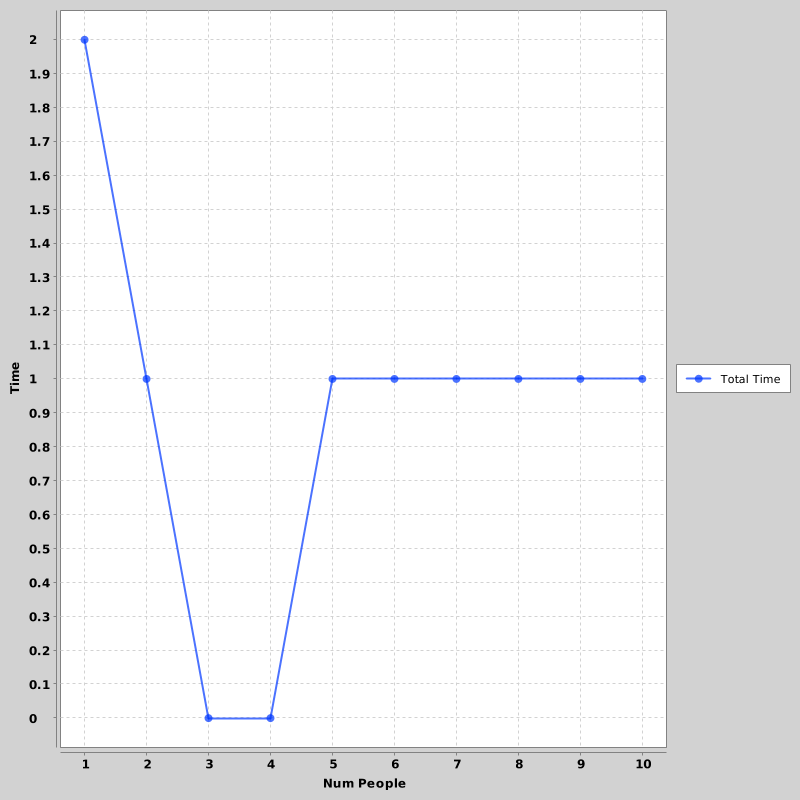
\includegraphics[scale=0.4]{numpeople-vs-time(split-for-unvisited)}
				\caption{number of people vs time taken to solve maze for a modified solution where splitting only occurs when a junction has multiple unvisited paths}
			\end{figure}
			
			The variance in the graph is very high, so there is no clear trend. This is caused because we are randomly selecting a path to take. But even with this large amount of variance we can immediately see two things. Firstly the overall performance is drastically improved compared to the previous solution. And secondly we don't get an exponential increase in time as we increase the number of people. If anything this graph indicates that the running time stays about the same as the data points are all varied around the same region. Given this performance increase we can make the maximum number of people larger and examine that graph
			
			\begin{figure}[H]
				\centering
				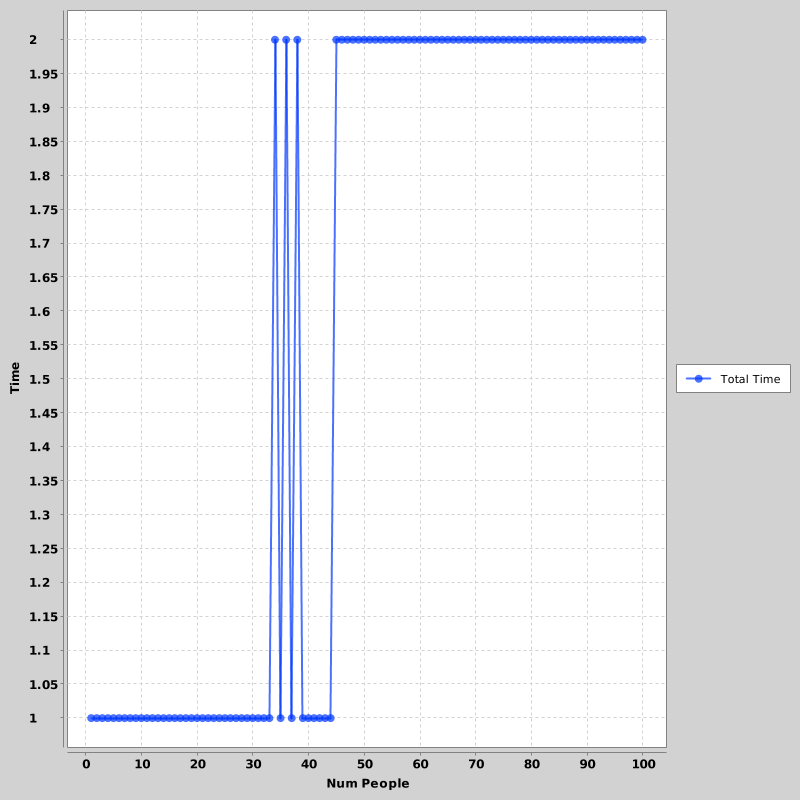
\includegraphics[scale=0.4]{numpeople-vs-time(split-for-unvisted)2}
				\caption{Same as Figure 2 but with a larger max number of people}
			\end{figure}
			
			This new graph which goes up to a party size of 100 still has a lot of variance but we can see a trend, Like for the original solution the time taken increases as the number of people does but the growth of time taken is not nearly as fast as the original solution. Given these results we will keep this modification.
			
			We should note that before it was discussed that if we only have one person in our party then at junctions with no unvisited paths we should make random decision. This modification is just a more general version of that.
		
		\subsection{Calling Out}
			When a solution is found, we have to wait for all the search party's which are wandering around to find the the a cell with a Golden marking and follow it to the finished.\\
			
			A way to ensure party's immediately start moving towards the solution path once a solution has been found is to install a speaker system in the maze. So then when a group finishes they can tell everyone in the maze a solution has been found. Then if every search party re traces there steps by looking at what cell we used to arrive at the current, eventually they will arrive at the start. And we know that the path to finish will be retraced to the start as well. So we can compare the performance with and without this addition.
			
			\begin{figure}[H]
			\minipage{0.48\textwidth}
  				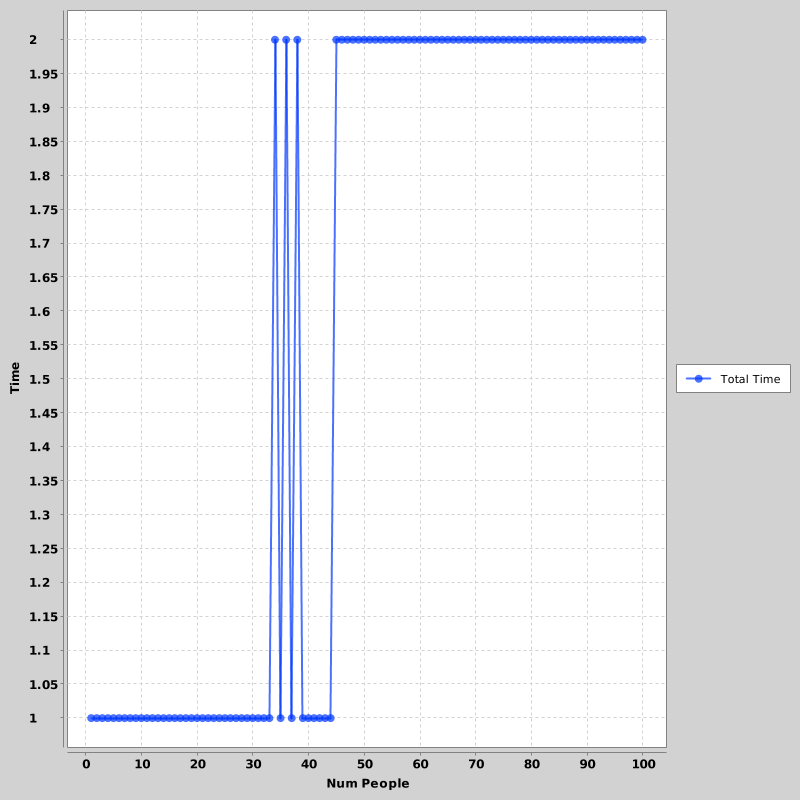
\includegraphics[width=\linewidth]{numpeople-vs-time(split-for-unvisted)2}
  				\caption{Without calling out}
			\endminipage\hfill
			\minipage{0.48\textwidth}
  				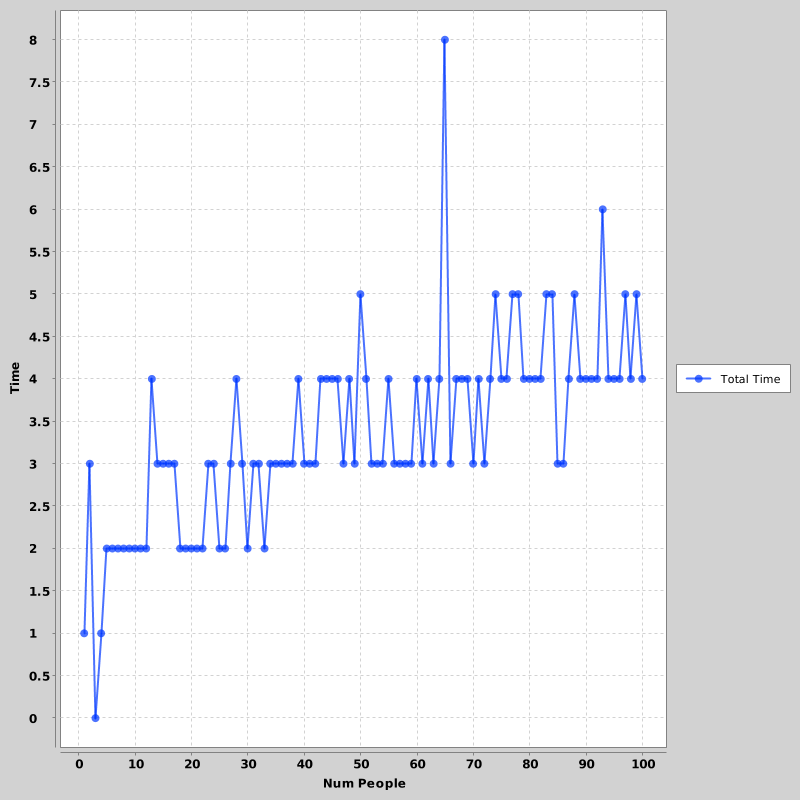
\includegraphics[width=\linewidth]{numpeople-vs-time(with-callingout)}
  				\caption{With calling out}
				\endminipage\hfill
			\end{figure}			
	
			Comparing these graphs show that this modification actually causes a noticeable performance decrease, for this reason we will disregard this modification.
		
	
	\section{Final Solution Analysis}  	
		To get a better idea of the performance of this solution we want to test it across a number of machines each with a different number of cores and core speed. The following 4 computers are what we will use.
		
		\begin{enumerate}
			\item \textbf{Home PC 1:} Has 1 core, and 1 thread per core. Total of 1 CPU's running at 2.7GHz
			
			\item \textbf{Home Laptop:} Has 2 cores, and 2 threads per core. Total of 4 CPU's running at 1.6GHz
			
			\item \textbf{Home PC 2:} Has 4 cores, and 2 threads per core. Total of 8 CPU's running at 3.5GHz
			
			\item \textbf{Lighthouse:} Has 64 CPU's
		\end{enumerate}
		
		\begin{figure}[H]
			\minipage{0.48\textwidth}
  				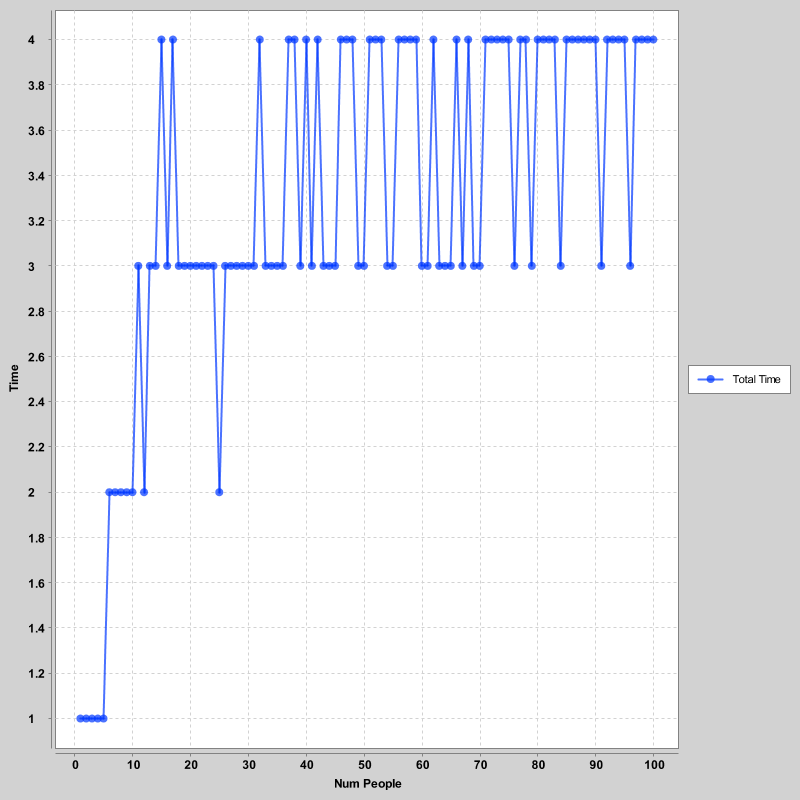
\includegraphics[width=\linewidth]{numpeople-vs-time(homepc1)}
  				\caption{Program run on home pc 1}
			\endminipage\hfill
			\minipage{0.48\textwidth}
  				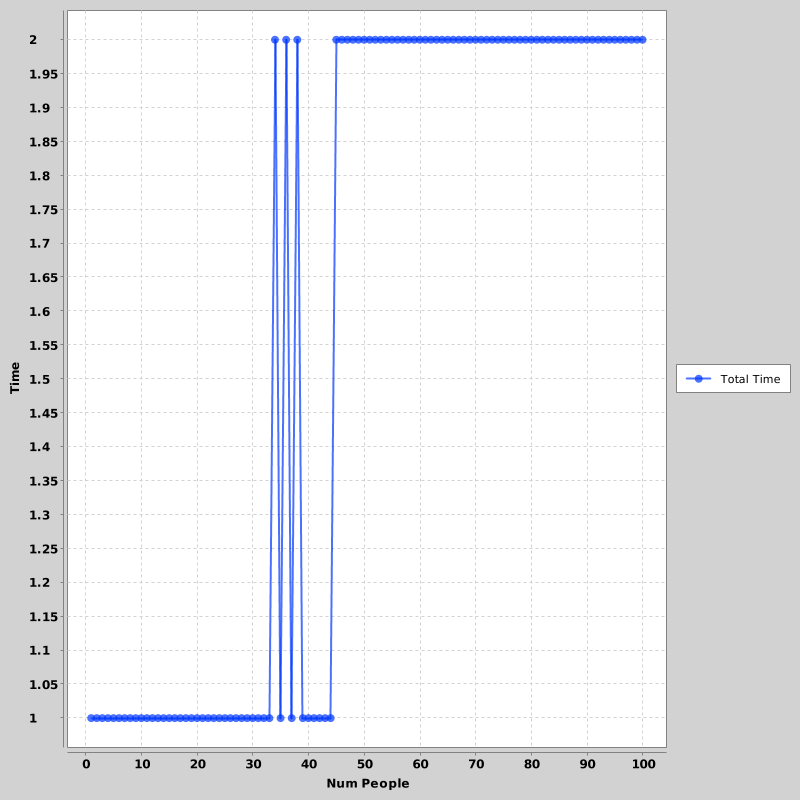
\includegraphics[width=\linewidth]{numpeople-vs-time(split-for-unvisted)2}
  				\caption{Program run on home laptop}
				\endminipage\hfill
		\end{figure}
			
		\begin{figure}[H]
			\minipage{0.48\textwidth}
  				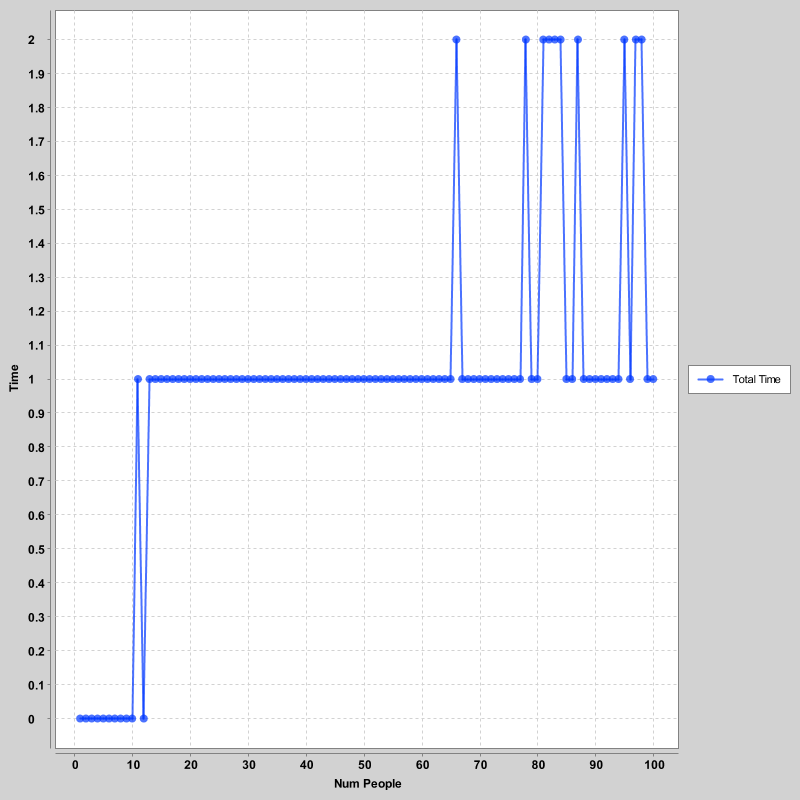
\includegraphics[width=\linewidth]{numpeople-vs-time(homepc2)}
  				\caption{Program run on home pc 2}
			\endminipage\hfill
			\minipage{0.48\textwidth}
  				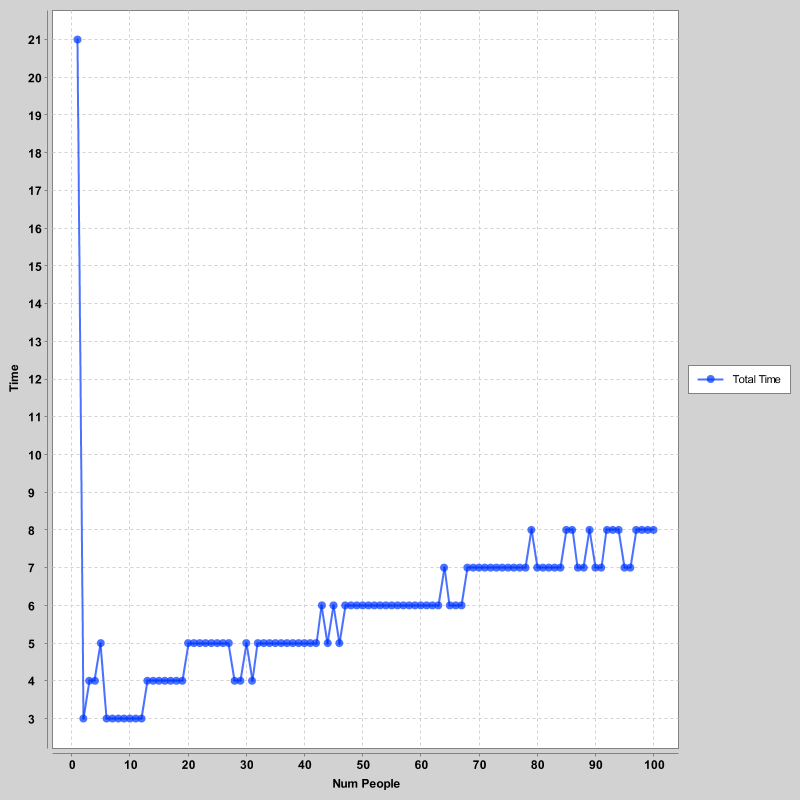
\includegraphics[width=\linewidth]{numpeople-vs-time(lighthouse)}
  				\caption{Program run on lighthouse}
				\endminipage\hfill
		\end{figure}
					
		We see the graphs for home pc 1, home laptop and home pc 2 are all very similar, they all have the same shape. The interesting thing to notice here is that lighthouse performs worse than all of them despite having a lot more cores. This indicates that we aren't utilizing the number of cores lighthouse has to offer. We run lighthouse, home pc 1 and home pc 2 over a new maze of size 40
		
		\begin{figure}[H]
			\minipage{0.48\textwidth}
  				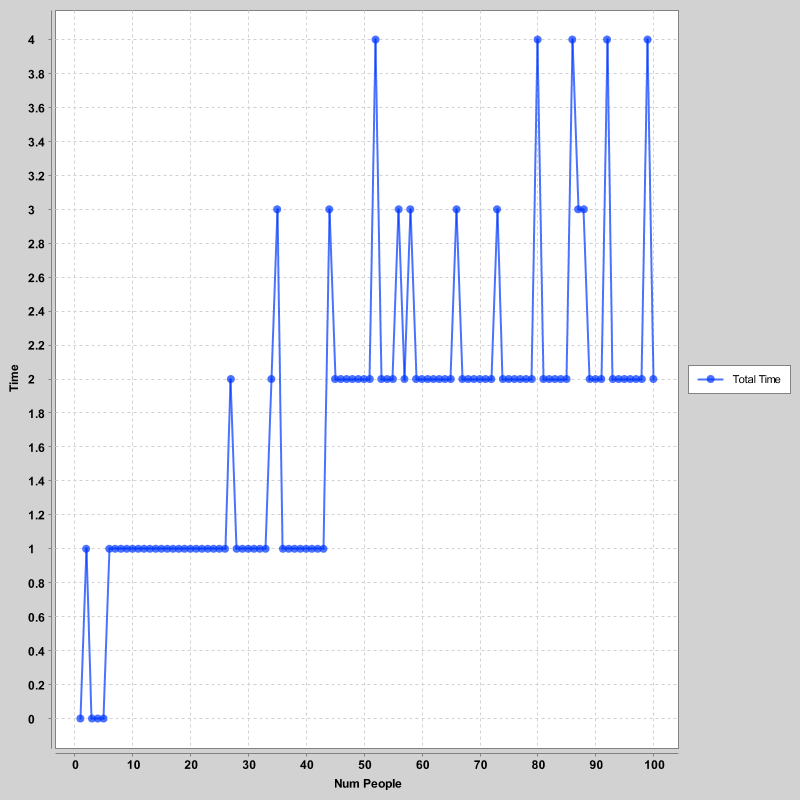
\includegraphics[width=\linewidth]{numpeople-vs-time(homepc2-big)}
  				\caption{Program run on home pc 2 with size 40 maze}
			\endminipage\hfill
			\minipage{0.48\textwidth}
  				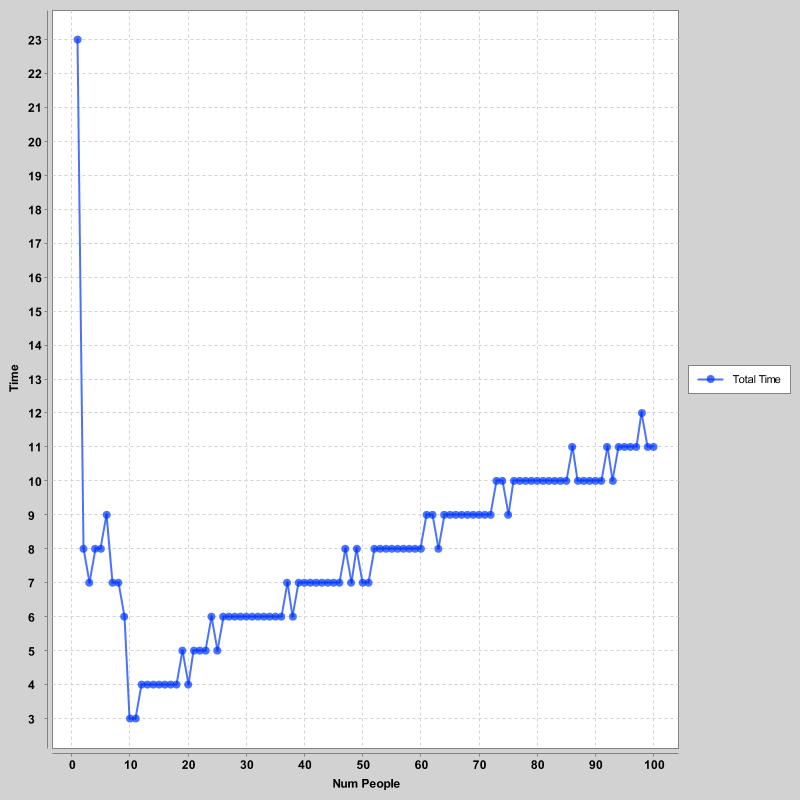
\includegraphics[width=\linewidth]{numpeople-vs-time(lighthouse-big)}
  				\caption{Program run on lighthouse with size 40 maze}
			\endminipage\hfill
		\end{figure}
		
		\begin{figure}[H]
			\minipage{0.48\textwidth}
  				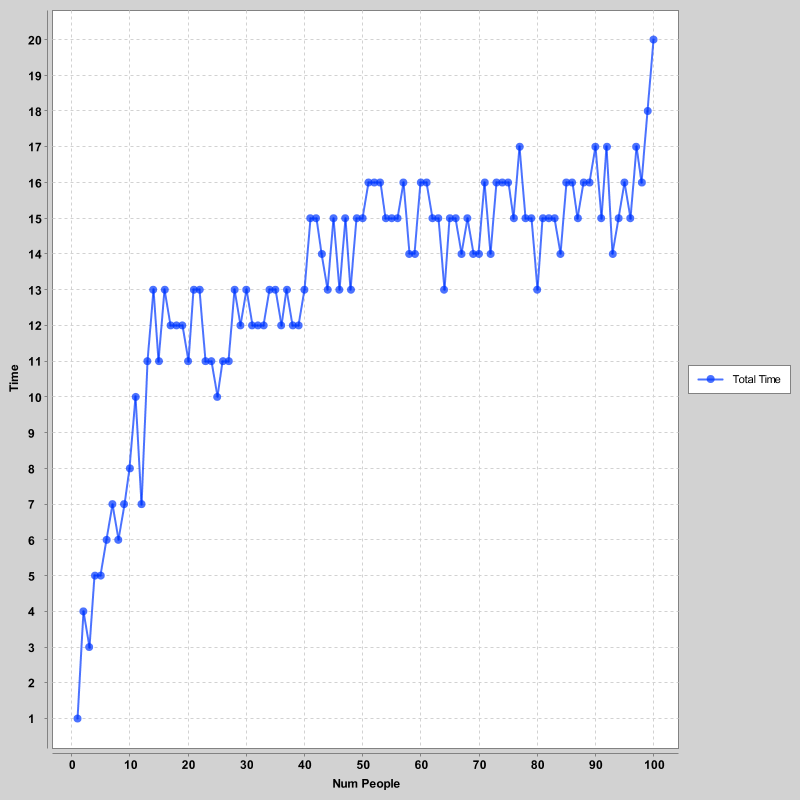
\includegraphics[width=\linewidth]{numpeople-vs-time(homepc1-big)}
  				\caption{Program run on home pc 1 with size 40 maze}
			\endminipage\hfill
		\end{figure}
		
		Here we see that lighthouse generally beats home pc 1 but performs a lot worse than home pc 2. This shows that despite the volume of cores lighthouse has, the processing power of home pc 2 gives it a better performance than lighthouse for this problem.
	
		\subsection{Real World}	
			However in real live we would expect the time taken to solve the maze to decrease as we increase the number of people, until we a point where we have enough people to explore every path so adding more people wont make a difference. At the moment we are seeing the opposite because of the overhead of each of the processes along with the locking methods. To attempt to simulate this better we could introduce a delay. A random delay between 0 and 10ms, this would represent it taking 0 to 10 mins for a search party make its move. We then run this on the home laptop machine with the maze of size 20
		
			\begin{figure}[H]
				\centering
				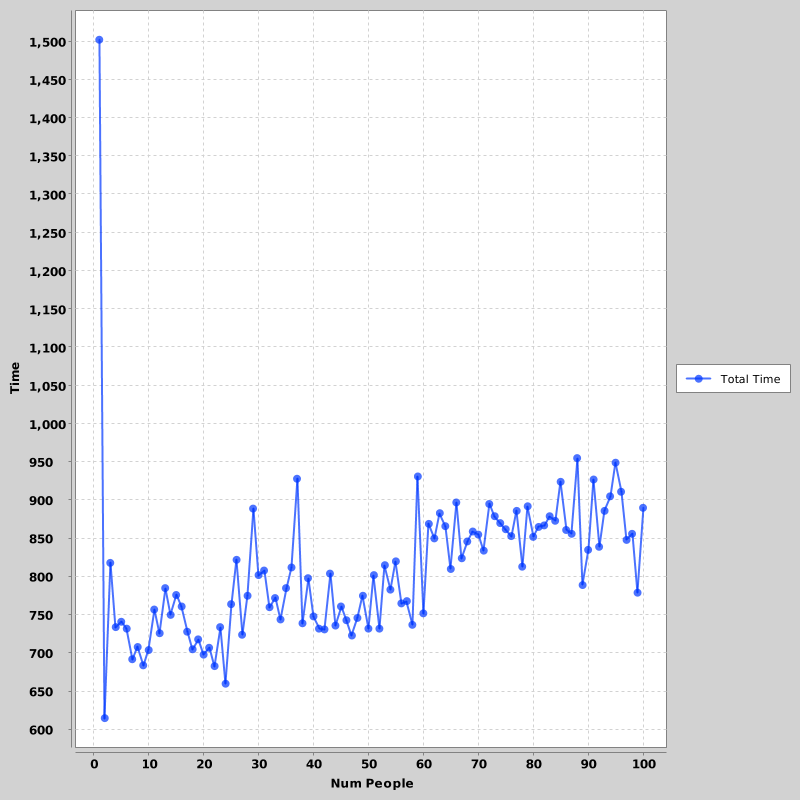
\includegraphics[scale=0.4]{numpeople-vs-time(home-laptop-w-delay)}
				\caption{Final solution run on home laptop but with a delay to simulate travel time}
			\end{figure}
	
			This still doesn't give us the result we expect, the time taken still trends upwards which is not what we would expect to happen
		
\end{document}